\documentclass{article}

%----------------------------------------------------------------------------------------
%	PACKAGES AND OTHER DOCUMENT CONFIGURATIONS
%----------------------------------------------------------------------------------------

\usepackage[T1]{fontenc}
\usepackage[utf8]{inputenc}
\usepackage{lmodern}
\usepackage[english]{babel}
\usepackage[autostyle]{csquotes}
\usepackage{graphicx} % Required for inserting images
\usepackage[hyphens]{url}
\usepackage{hyperref}
\usepackage{amsmath}      % for additional mathematical features
\usepackage{amsfonts}     % for mathbb command
\usepackage{float}
\usepackage{setspace}
\usepackage{listings}
\doublespacing
\usepackage[backend=biber,style=authoryear]{biblatex}
\renewcommand*{\bibfont}{\small}
\addbibresource{Bibliographie.bib}
\usepackage{tcolorbox}

%----------------------------------------------------------------------------------------
%	DOCUMENT MARGINS
%----------------------------------------------------------------------------------------

\usepackage{geometry} % Required for adjusting page dimensions and margins

\geometry{
	paper=a4paper, % Paper size, change to letterpaper for US letter size
	top=3cm, % Top margin
	bottom=3cm, % Bottom margin
	left=3cm, % Left margin
	right=3cm, % Right margin
	headheight = 10pt, % Header height
	footskip = 1.5cm, % Space from the bottom margin to the baseline of the footer
	headsep = 1.2cm, % Space from the top margin to the baseline of the header
	%showframe, % Uncomment to show how the type block is set on the page
}

\title{Kohyama model parametrisation for 5 species}
\author{Clementine de Montgolfier}
\date{Nov 2023}

\begin{document}

\maketitle

\section{Model parametrisation}

We are starting with a 3 layers 3 species system with a mixture of possible species oak, beech, pine, epicea, hetre, and 3 layers of dbh (cm) interval [0,27.5], [27.5,67.5], [67.5+[. We have to define all parameters in Table \ref{tab:coeftoparam}.

\begin{table}[H]
    \centering
    \begin{tabular}{l l l}
    \hline
    \hline
    \multicolumn{3}{l}{\textbf{By species}, $sp$} \\
    \hline
    $b_{sp,1}$     & optimal birth probability per tree in layer $L$ & $year^{-1}$ \\
    $Cb_{sp,1}$    & birth susceptibility to superior foliage density& \\
    \\
    \multicolumn{3}{l}{\textbf{By species $sp$ and layer $l$}} \\
    \hline
    $\phi_{sp,l}$  & foliage density per tree of species $sp$ in layer $l$  & $ha^{-1}$  \\
    $m_{sp,l}$     & probability of intrinsic mortality                     & $ha^{-1}.year^{-1}$ \\  
    $g_{sp,l}$     & optimal probability of transition from layer $l$ to the next   & $.year^{-1}$ \\
    $Cg_{sp,l}$    & growth susceptibility to superior foliage density      &            \\
    $Cm_{sp,l}$    & mortality susceptibility to superior foliage density   &            \\
    \hline
    \hline
    \end{tabular}
    \caption{Parameters that we have to define numerically}
    \label{tab:coeftoparam}
\end{table}

FORCEEPS simulations where used to adjust the dynamic of the system. 5 species where chosen to do so : Quercus petraea, Fagus sylvatica, Pinus sylvestris, Picea abies, and Abies alba. We chose a constant climate for 300 years drawn randomly from meteorologic data from Bern between 1950 and 2000 (resulting climate can be found in Fig. Appendix). We used 2 initial states. Parameters of the system were adjusted on the resulting dynamics.\\

\section{Parameters deduced form litterature of Forceeps and ForClim}

\subsection{Intrinsec Mortality}

Mortality was defined axactly as in Forceeps, as the inverse of the life expectancy of the species ($A_{max}$) multiplied by a factor $c_{mort}$ = 4.605.
\begin{equation}
    m_s = \frac{c_{mort}}{A_{max_s}}
\end{equation}

$A_max$ can be found in the appendix (REF Bugmann)

\subsection{Optimal Growth}

Optimal growth is defined in forceeps as :

\begin{equation}
    \Delta D_{\mathrm{opt}_i}(t+1)=g_s \frac{D_i(t)\left(1-\frac{H_i(t)}{H_{\max _s}}\right)}{2 H_{\max _s}-b_{\max _s} \times \exp \left(\left(\frac{-s_s}{b_{\max _s}} D_i(t)\right) \times\left(\frac{-s_s}{b_{\max _s}} D_i(t)+2\right)\right.}
\end{equation}

With $g_s$ the growth rate, $D_i$ the diameter of the tree, $H_i$ the height of the tree, $H_{\max _s}$ the maximum height of the species, $b_{\max _s}$ the maximum heigth of the species above breast ($b_{\max _s} =  H_{\max _s} - 1.37$), and $s_s$ the shape parameter of the species. $g_s$, $H_{\max _s}$, and $s_s$ can be found in the appendix (REF Bugmann). $H_i$ is also defined as a function of $D_i$ :

\begin{equation}
    H_i(t)=b+b_{\max _s}\left(1-\exp \left(-\frac{s_s}{b_{\max _s}} D_i(t)\right)\right)
\end{equation}

This gives a function $f(D_i) = \Delta D_{\mathrm{opt}_i}(t+1)$, which is the growth of the tree as a function of its diameter.
%insert figure : Growth_diameter.png

\begin{figure}
    \centering
    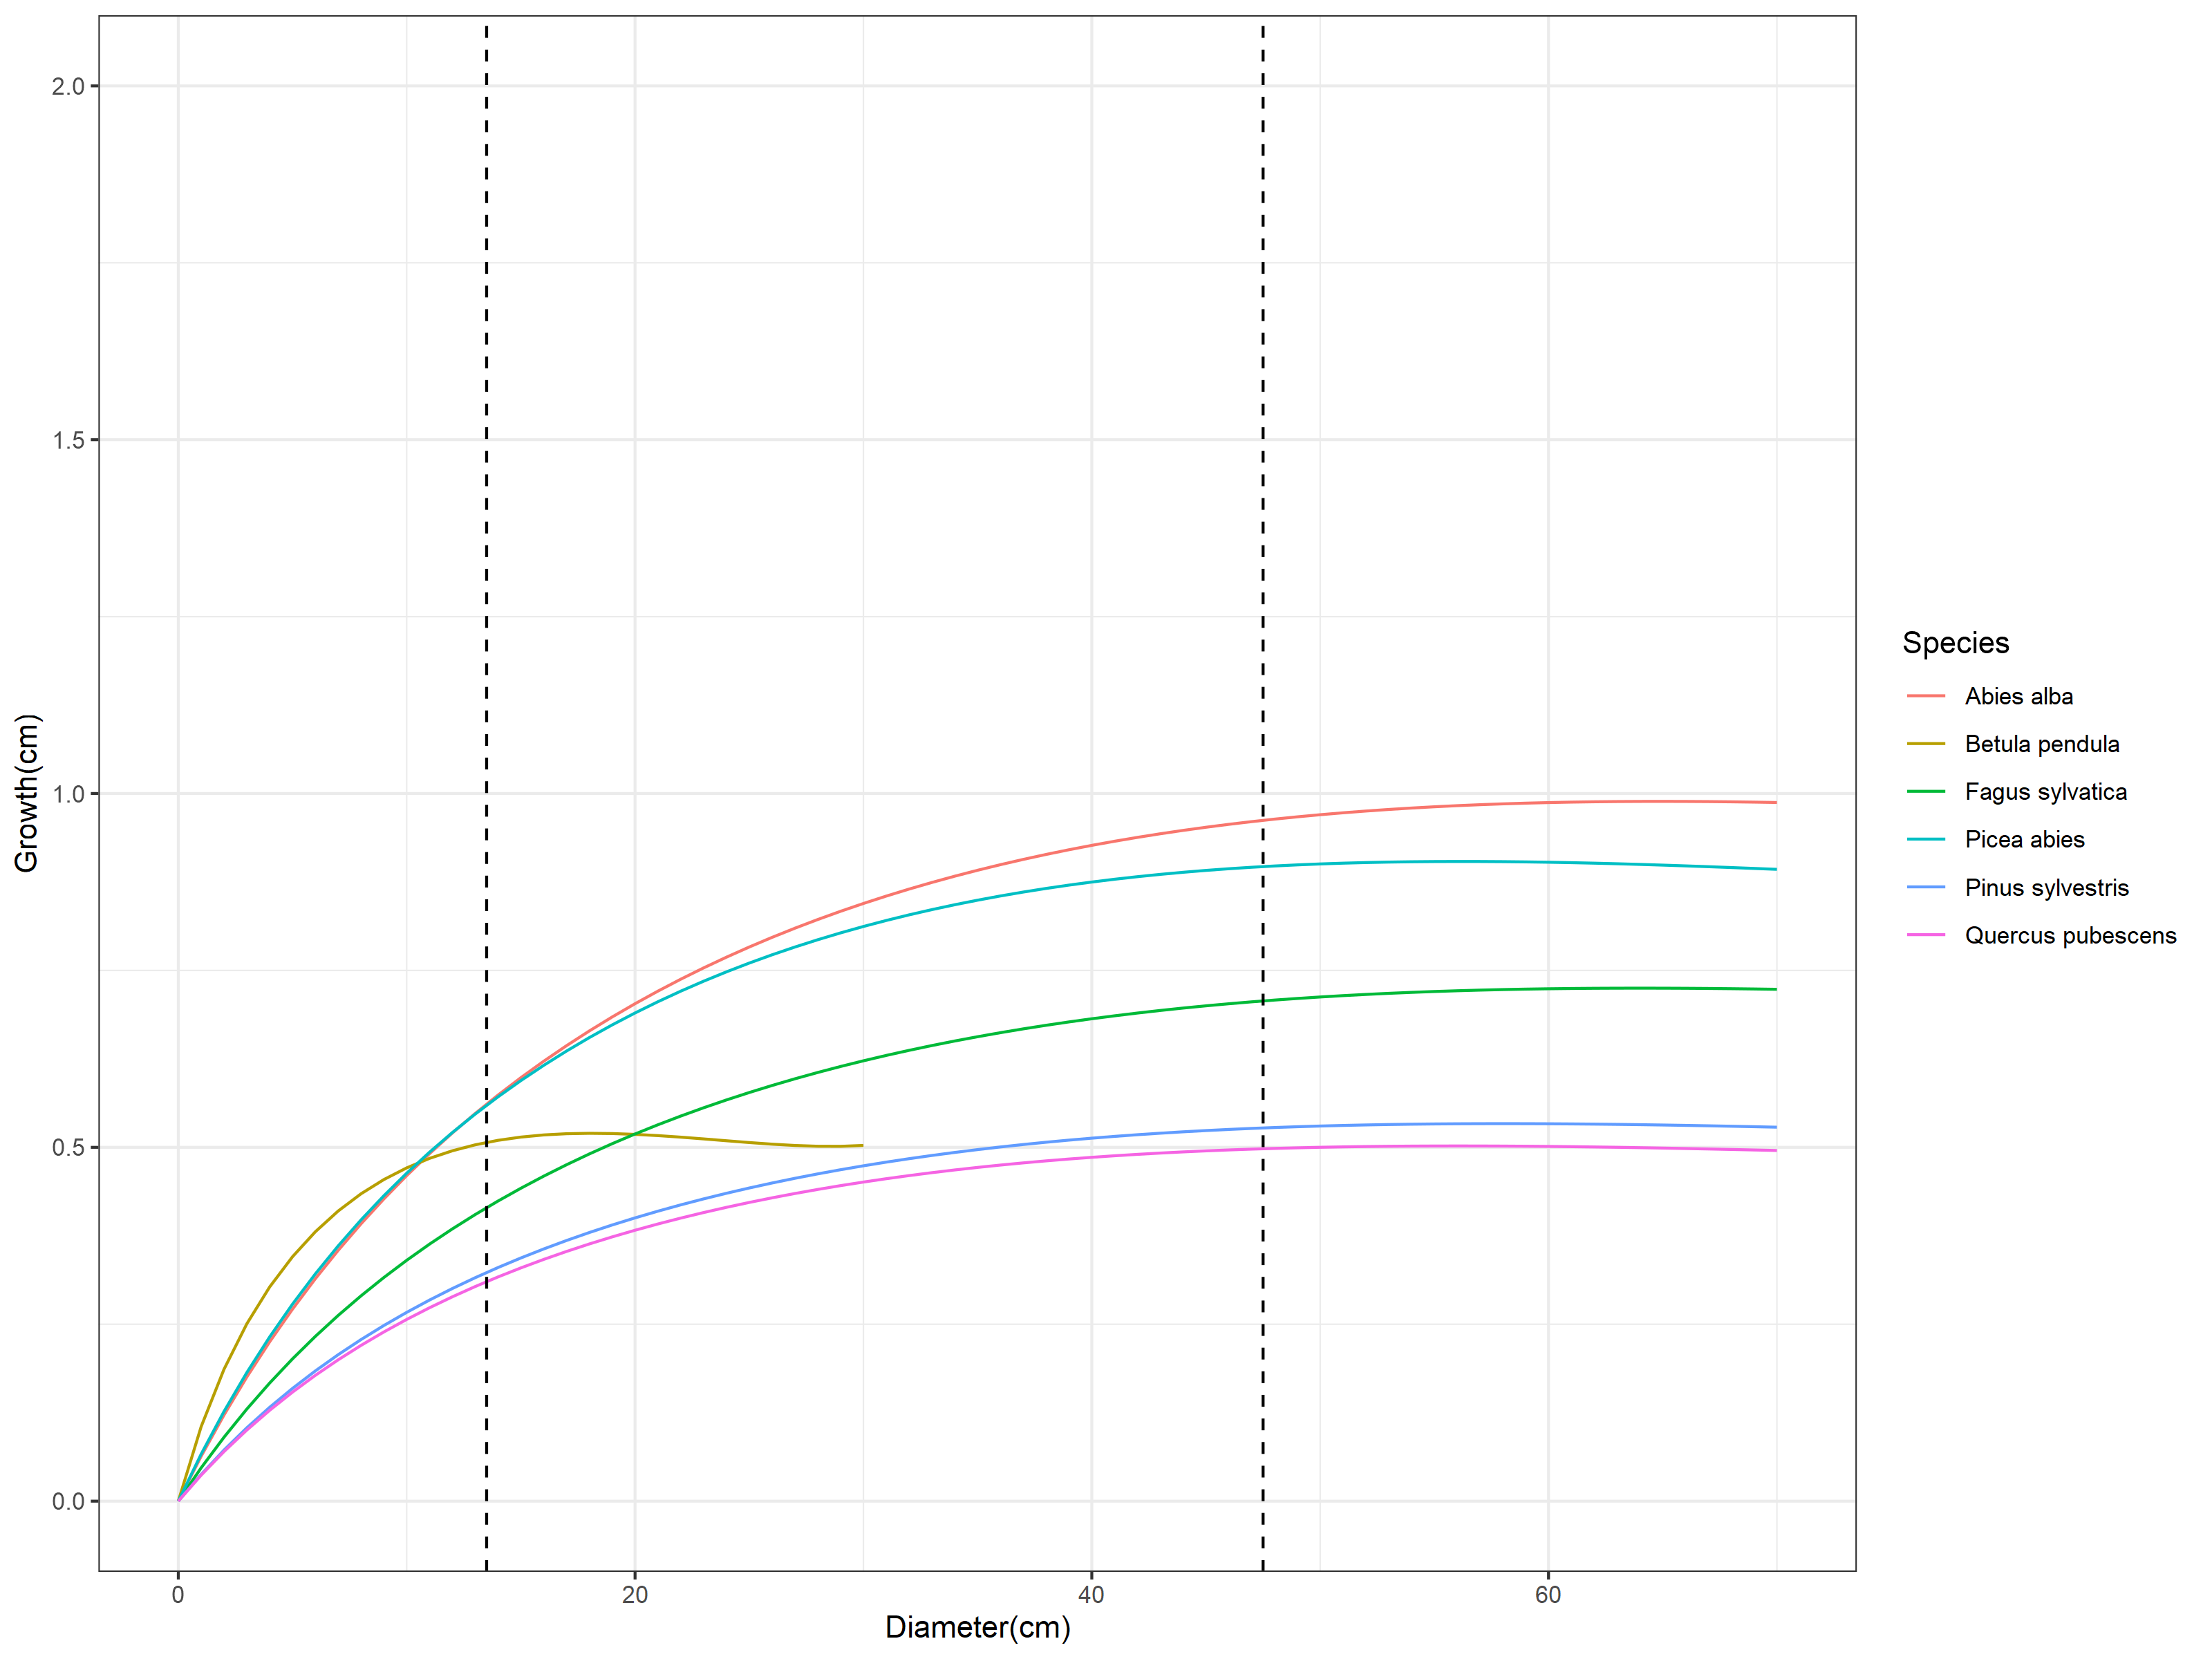
\includegraphics[width=0.8\textwidth]{Figure/Growth_diameter.png}
    \caption{Growth as a function of diameter for the 5 species}
    \label{fig:my_label}
\end{figure}

As our model does not account for a change of growth with diameter we took the growth from the mean diameter of our two interval : [0, 27.5] and [27.5, 67.5] (i.e. 13.75 and 47.5). It gives :

\begin{table}[H]
\begin{center}
    \begin{tabular}{lll}
    \hline
    Species & Growth 1 & Growth 2 \\ \hline
    \textit{Abies alba} & 0.5 & 0.96 \\
    \textit{Betula pendula} & 0.5 & 0 \\
    \textit{Fagus sylvatica} & 0.37 & 0.71 \\
    \textit{Picea abies} & 0.5 & 0.9 \\
    \textit{Pinus sylvestris} & 0.29 & 0.53 \\
    \textit{Quercus pubescens} & 0.28 & 0.5 \\ \hline
    \end{tabular}
    \caption{Growth for the 5 species and two below layers}
\end{center}
\end{table}

Growth is the number of cm added to the diameter of the tree each year. To get the transition probability to the next layer we need to divide this value by the diameter difference of the layer (See table 3).

\subsection{Optimal Esthablishment}

Establishment is a process that is still not well understood. In Forceeps optimal establishment (if all the threshold for establishment are met) is the same for every species : 0.6 individu/m2/year. We will use this value for our model.

\subsection {Light competition}

Proportionality between the species is known (see Forclim Ly (growth) and La(birth)), as mortality due to light competition is due to the absence of growth we used the same proportionality.

\begin{table}[H]
\begin{center}
    \begin{tabular}{lll}
    \hline
    Species & Ly (growth, mortality) & La (birth) \\ \hline
    \textit{Abies alba} & 1 & 3 \\
    \textit{Betula pendula} & 5 & 5 \\
    \textit{Fagus sylvatica} & 9 & 3 \\
    \textit{Picea abies} & 9 & 7 \\
    \textit{Pinus sylvestris} & 1 & 3 \\
    \textit{Quercus pubescens} & 8 & 7 \\ \hline
    \end{tabular}
    \caption{Sensitivity for light competition}
\end{center}
\end{table}

If we have a relative sensitivy of our species to light availability we still have to get the global coefficient linked to this sensitivity for growth, birth and mortality. We cannot extract the parameters from a simplification as we used a negative linear function, whuich is not the case in the model. We will use the data from Forceeps to fit our parameters.

\section{Forceeps input data and results}

\subsection{Climate}

Climate was taken randomly for each months in the climate data from 1950 to 2000 (Bern), to get a constant climate.

\begin{figure}[H]
    \centering
    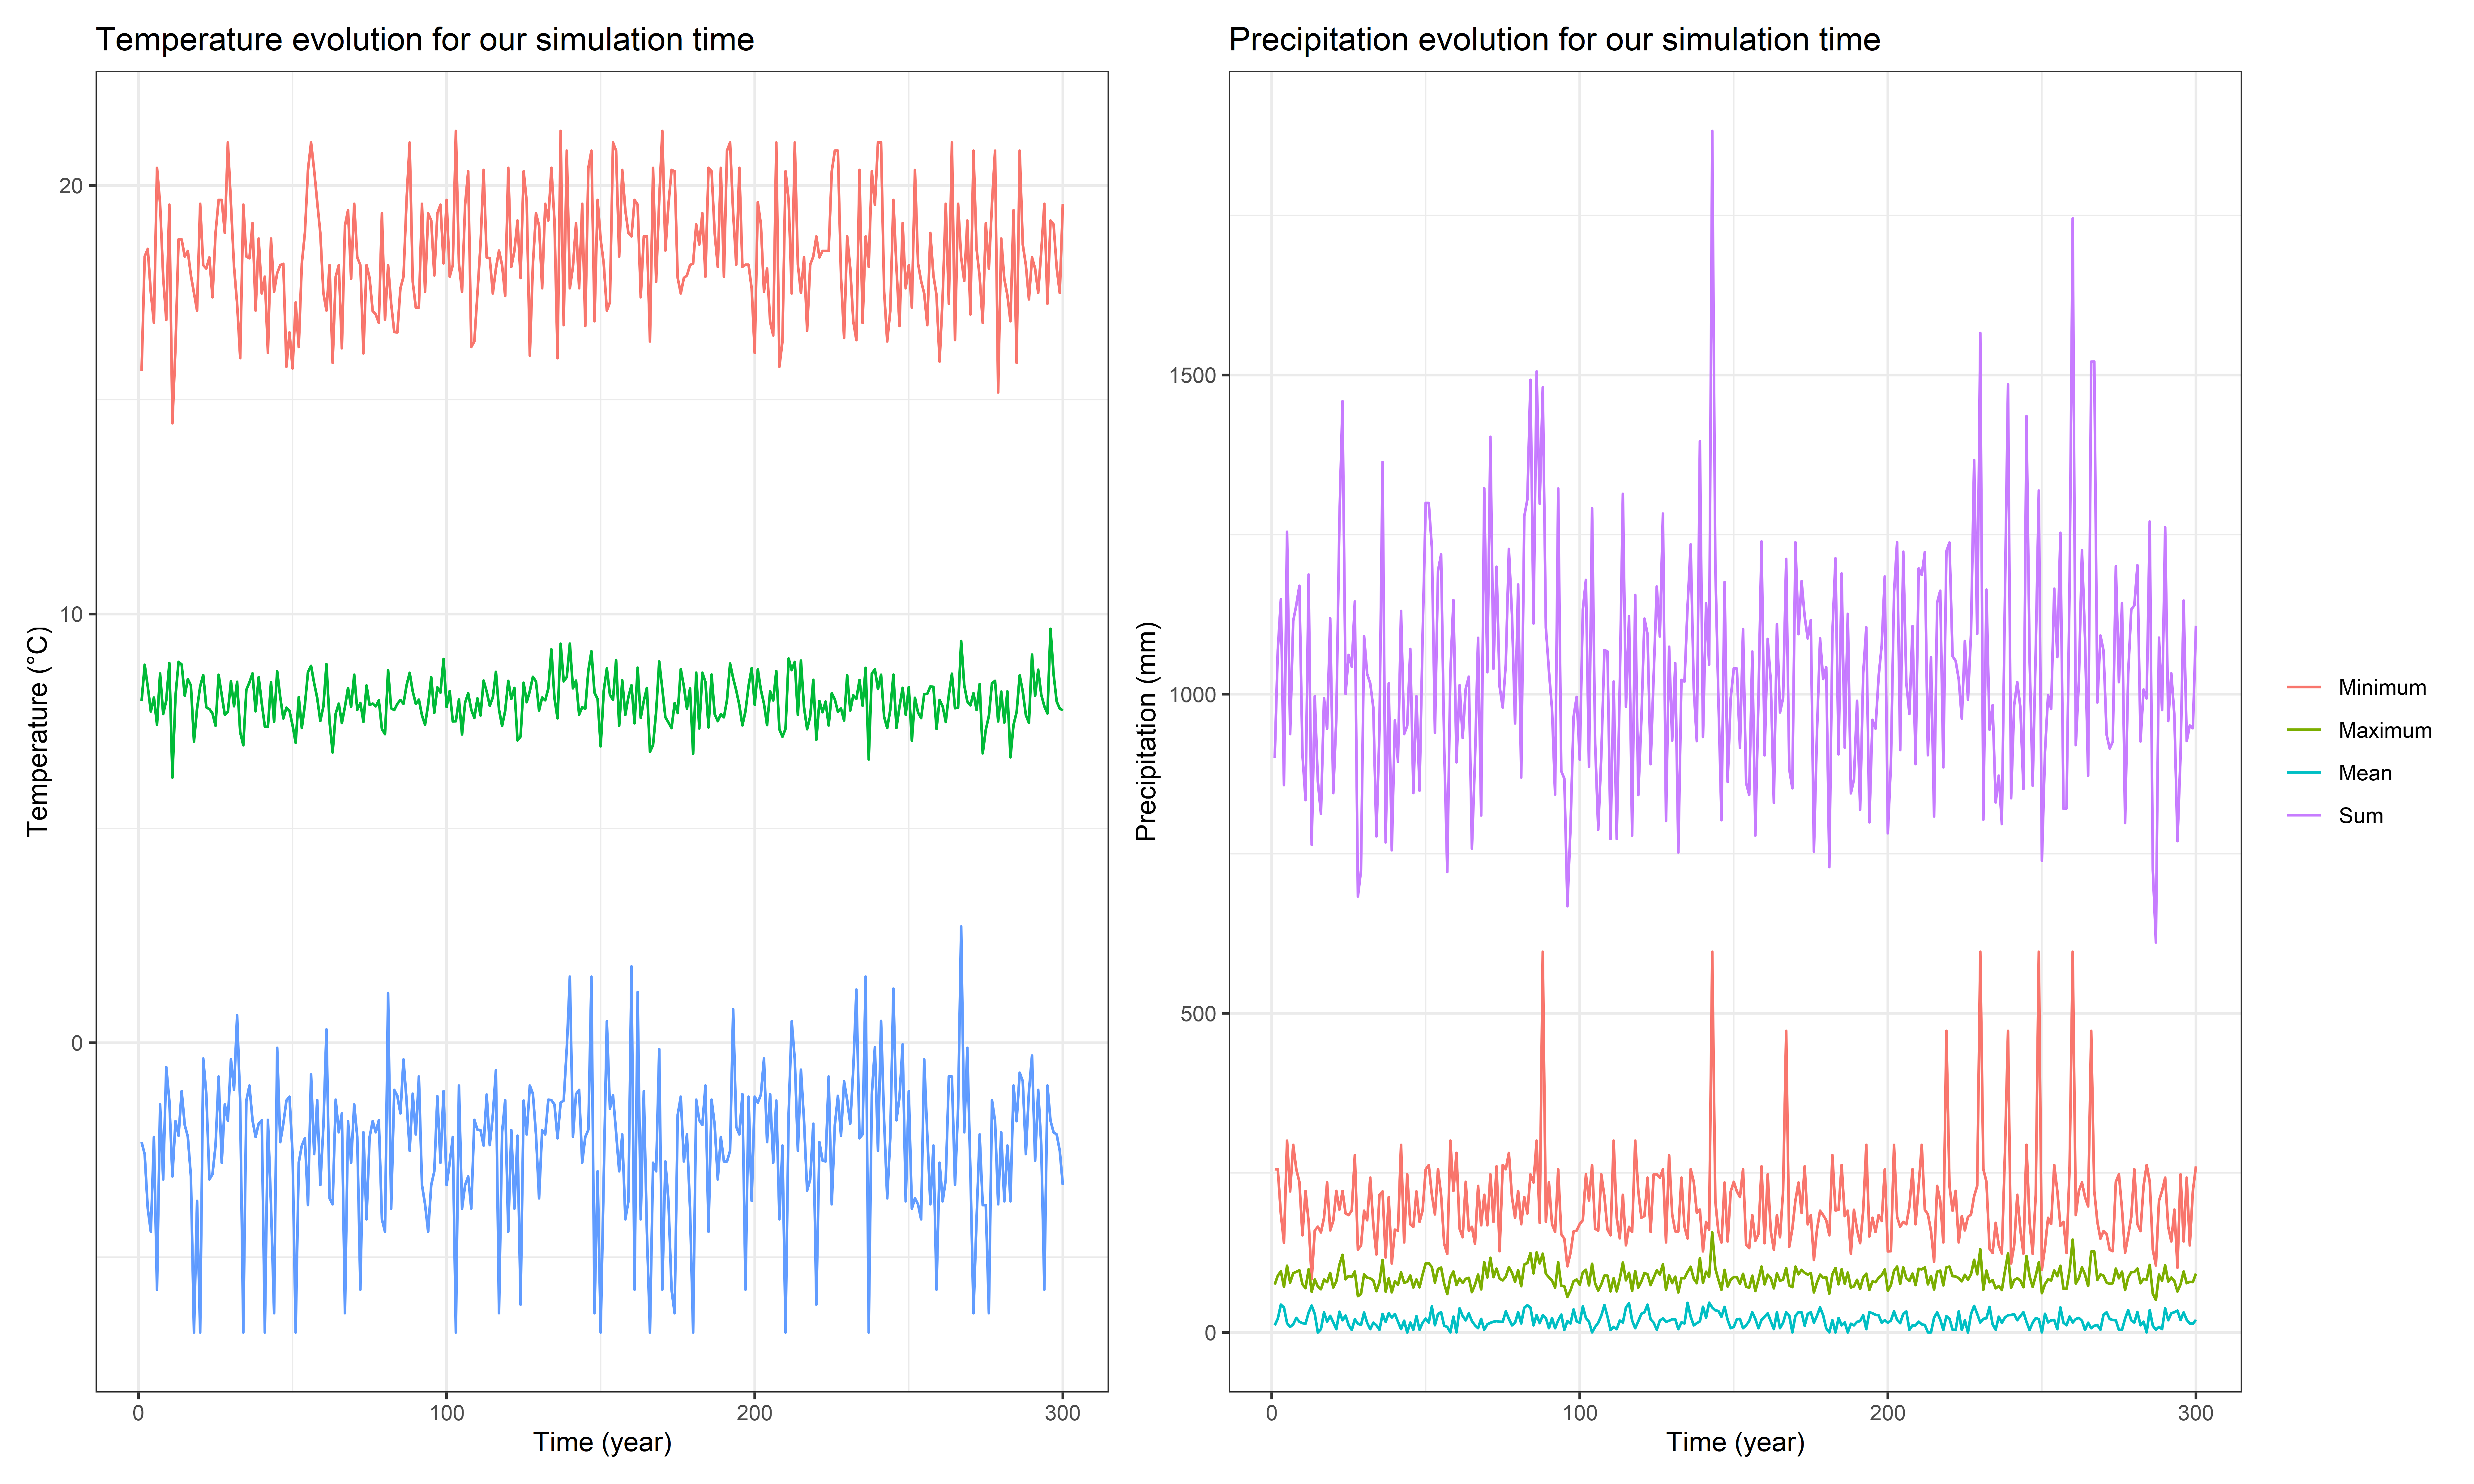
\includegraphics[width=0.8\textwidth]{Figure/Climate_simul.png}
    \caption{Climate for our ForCEEPS simulation}
    \label{fig:my_label}
\end{figure}

\subsubsection{setup parameters}

For the setup parameters xe used for the site : \\
siteBucketSize = 100 \\
siteAverageNitrogen = 100 \\
siteLatitude = 46.5 \\
siteLongitude = 7.5 \\
siteSlope = 0 \\
siteRegenerationForclimDensity = 0.006 \\
siteBrowsingDensity = 0 \\
siteMaxETPRate = 12 \\
siteFractionInterceptedPrec = 0.3 \\

And for basic setup :\\
regenerationForclimLike = true \\
establishmentProbabilityCoef = 0.1 \\

We did those analyses on 20 patches of 1000m2, result below are the mean of those 20 patches mulitiplied by 10 to be per hectare.

\section{Forceeps simulation}

Did two different initial forest structure, one with a random distribution of 10 trees in each layer and species.

\begin{figure}[H]
    \centering
    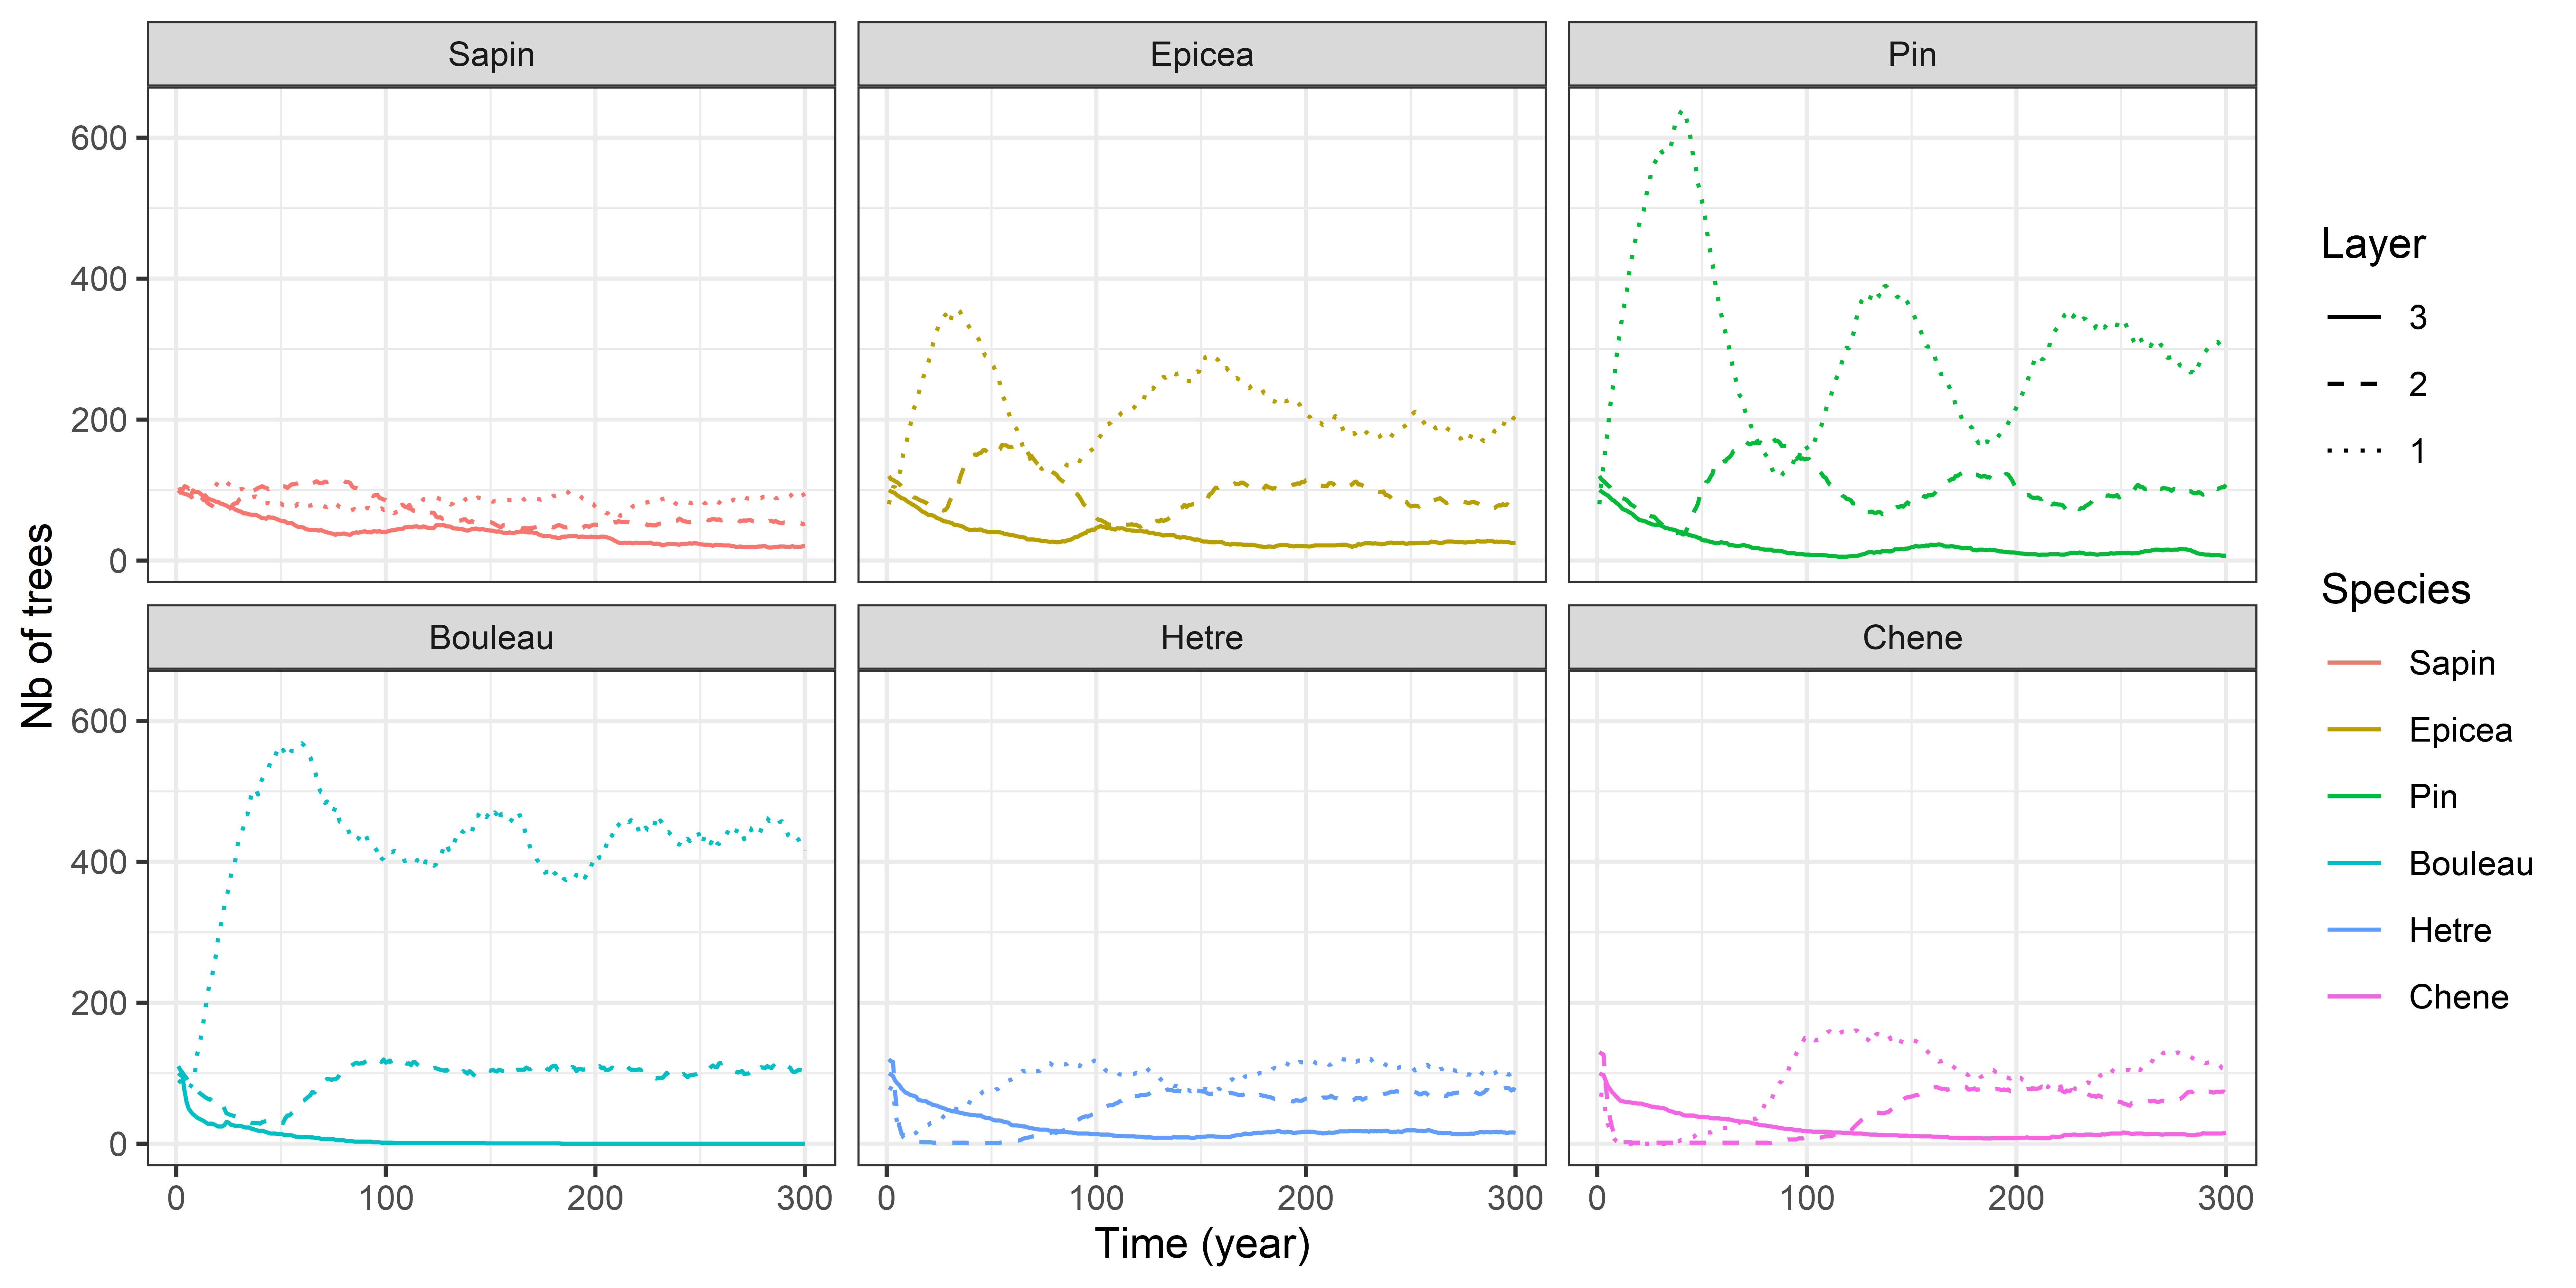
\includegraphics[width=0.8\textwidth]{Figure/forceps_simul_unique.png}
    \caption{ForCEEPS simulation for individual species}
    \label{fig:my_label}
\end{figure}

\begin{figure}[H]
    \centering
    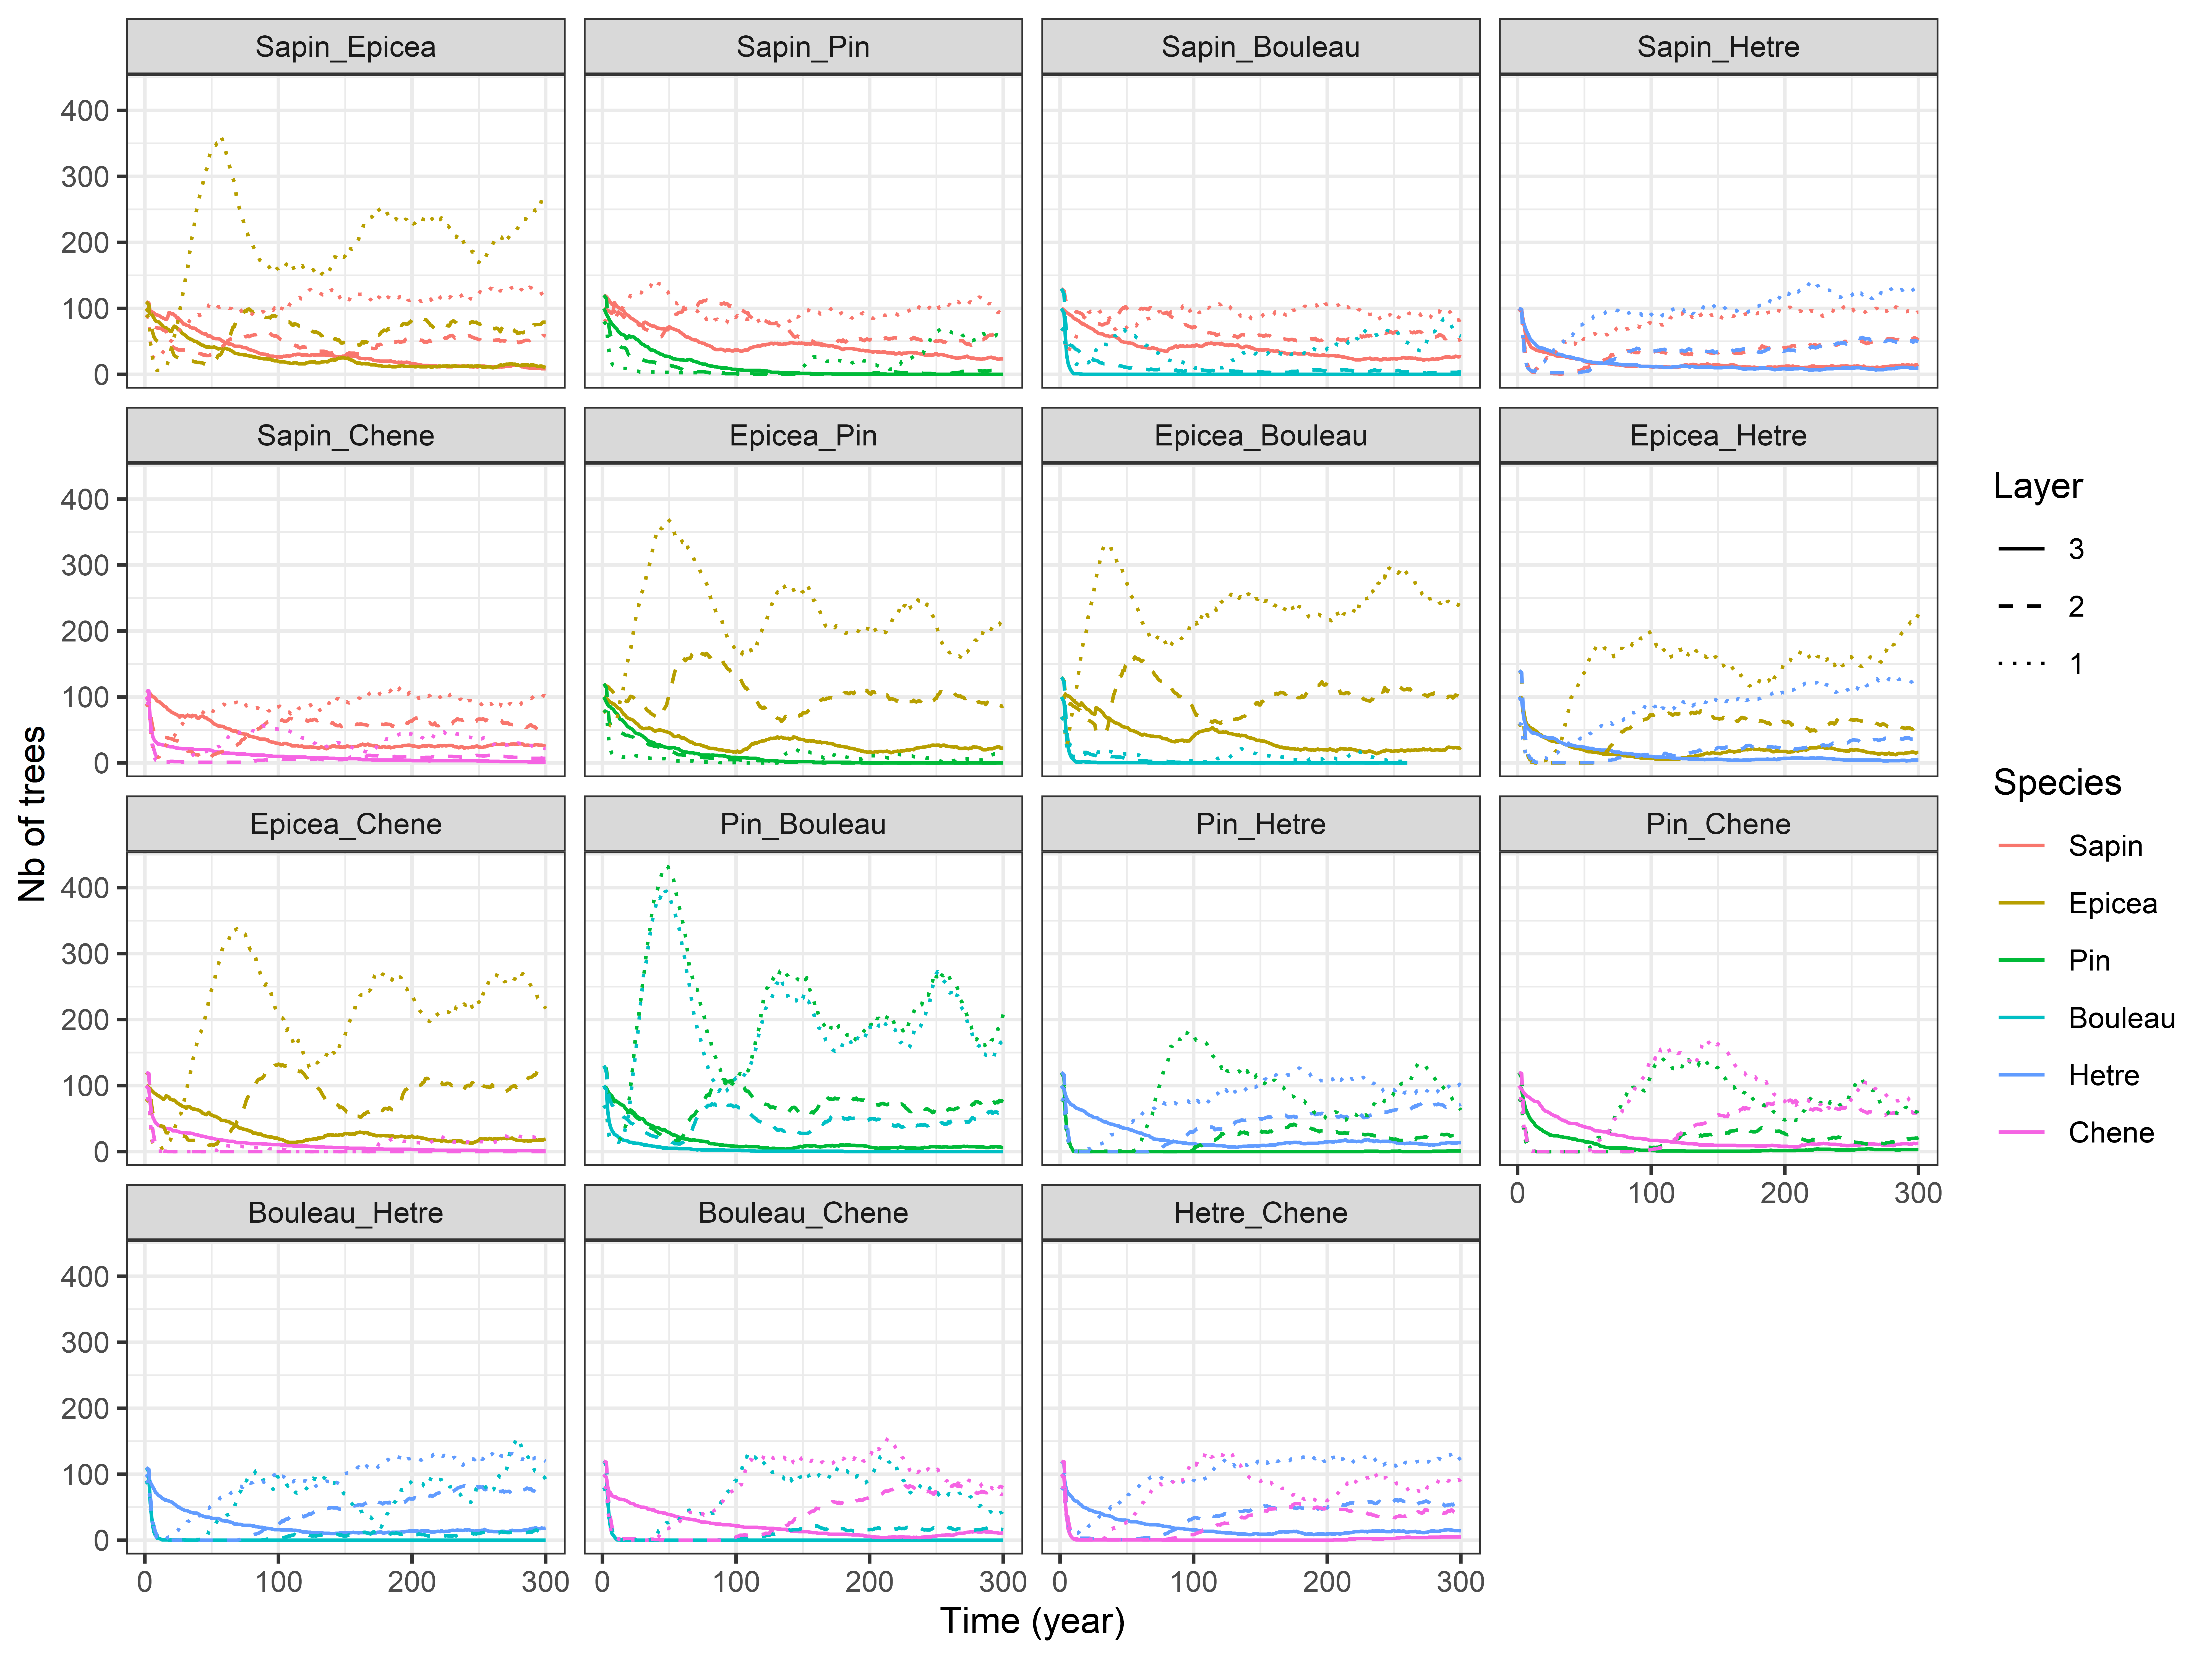
\includegraphics[width=0.8\textwidth]{Figure/forceps_simul_multi.png}
    \caption{ForCEEPS simulation for mixted species stand}
    \label{fig:my_label}
\end{figure}

\subsection{Fitting the parameters}

To fit the parameter we used the function optim in R with the following parameters :

\begin{tcolorbox}
result <- optimParallel(start point, function to minimize, lower = rep(0,3), upper = rep(0.1,3), method = ''L-BFGS-B'')
\end{tcolorbox}

Method "L-BFGS-B" (see optim documentation) allows box constraints, that is each variable can be given a lower and/or upper bound. The initial value must satisfy the constraints. This uses a limited-memory modification of the BFGS quasi-Newton method.  "BFGS" is a quasi-Newton method (also known as a variable metric algorithm), specifically that published simultaneously in 1970 by Broyden, Fletcher, Goldfarb and Shanno. This uses function values and gradients to build up a picture of the surface to be optimized.

I only fit three parameters LCg (light competition for growth), LCm (light competition for mortality) and LCb (light competition for birth). In the model they are then multiplied by the sensitivity of the species to light competition (see table 3).

\subsection{Results}

\begin{figure}[H]
    \centering
    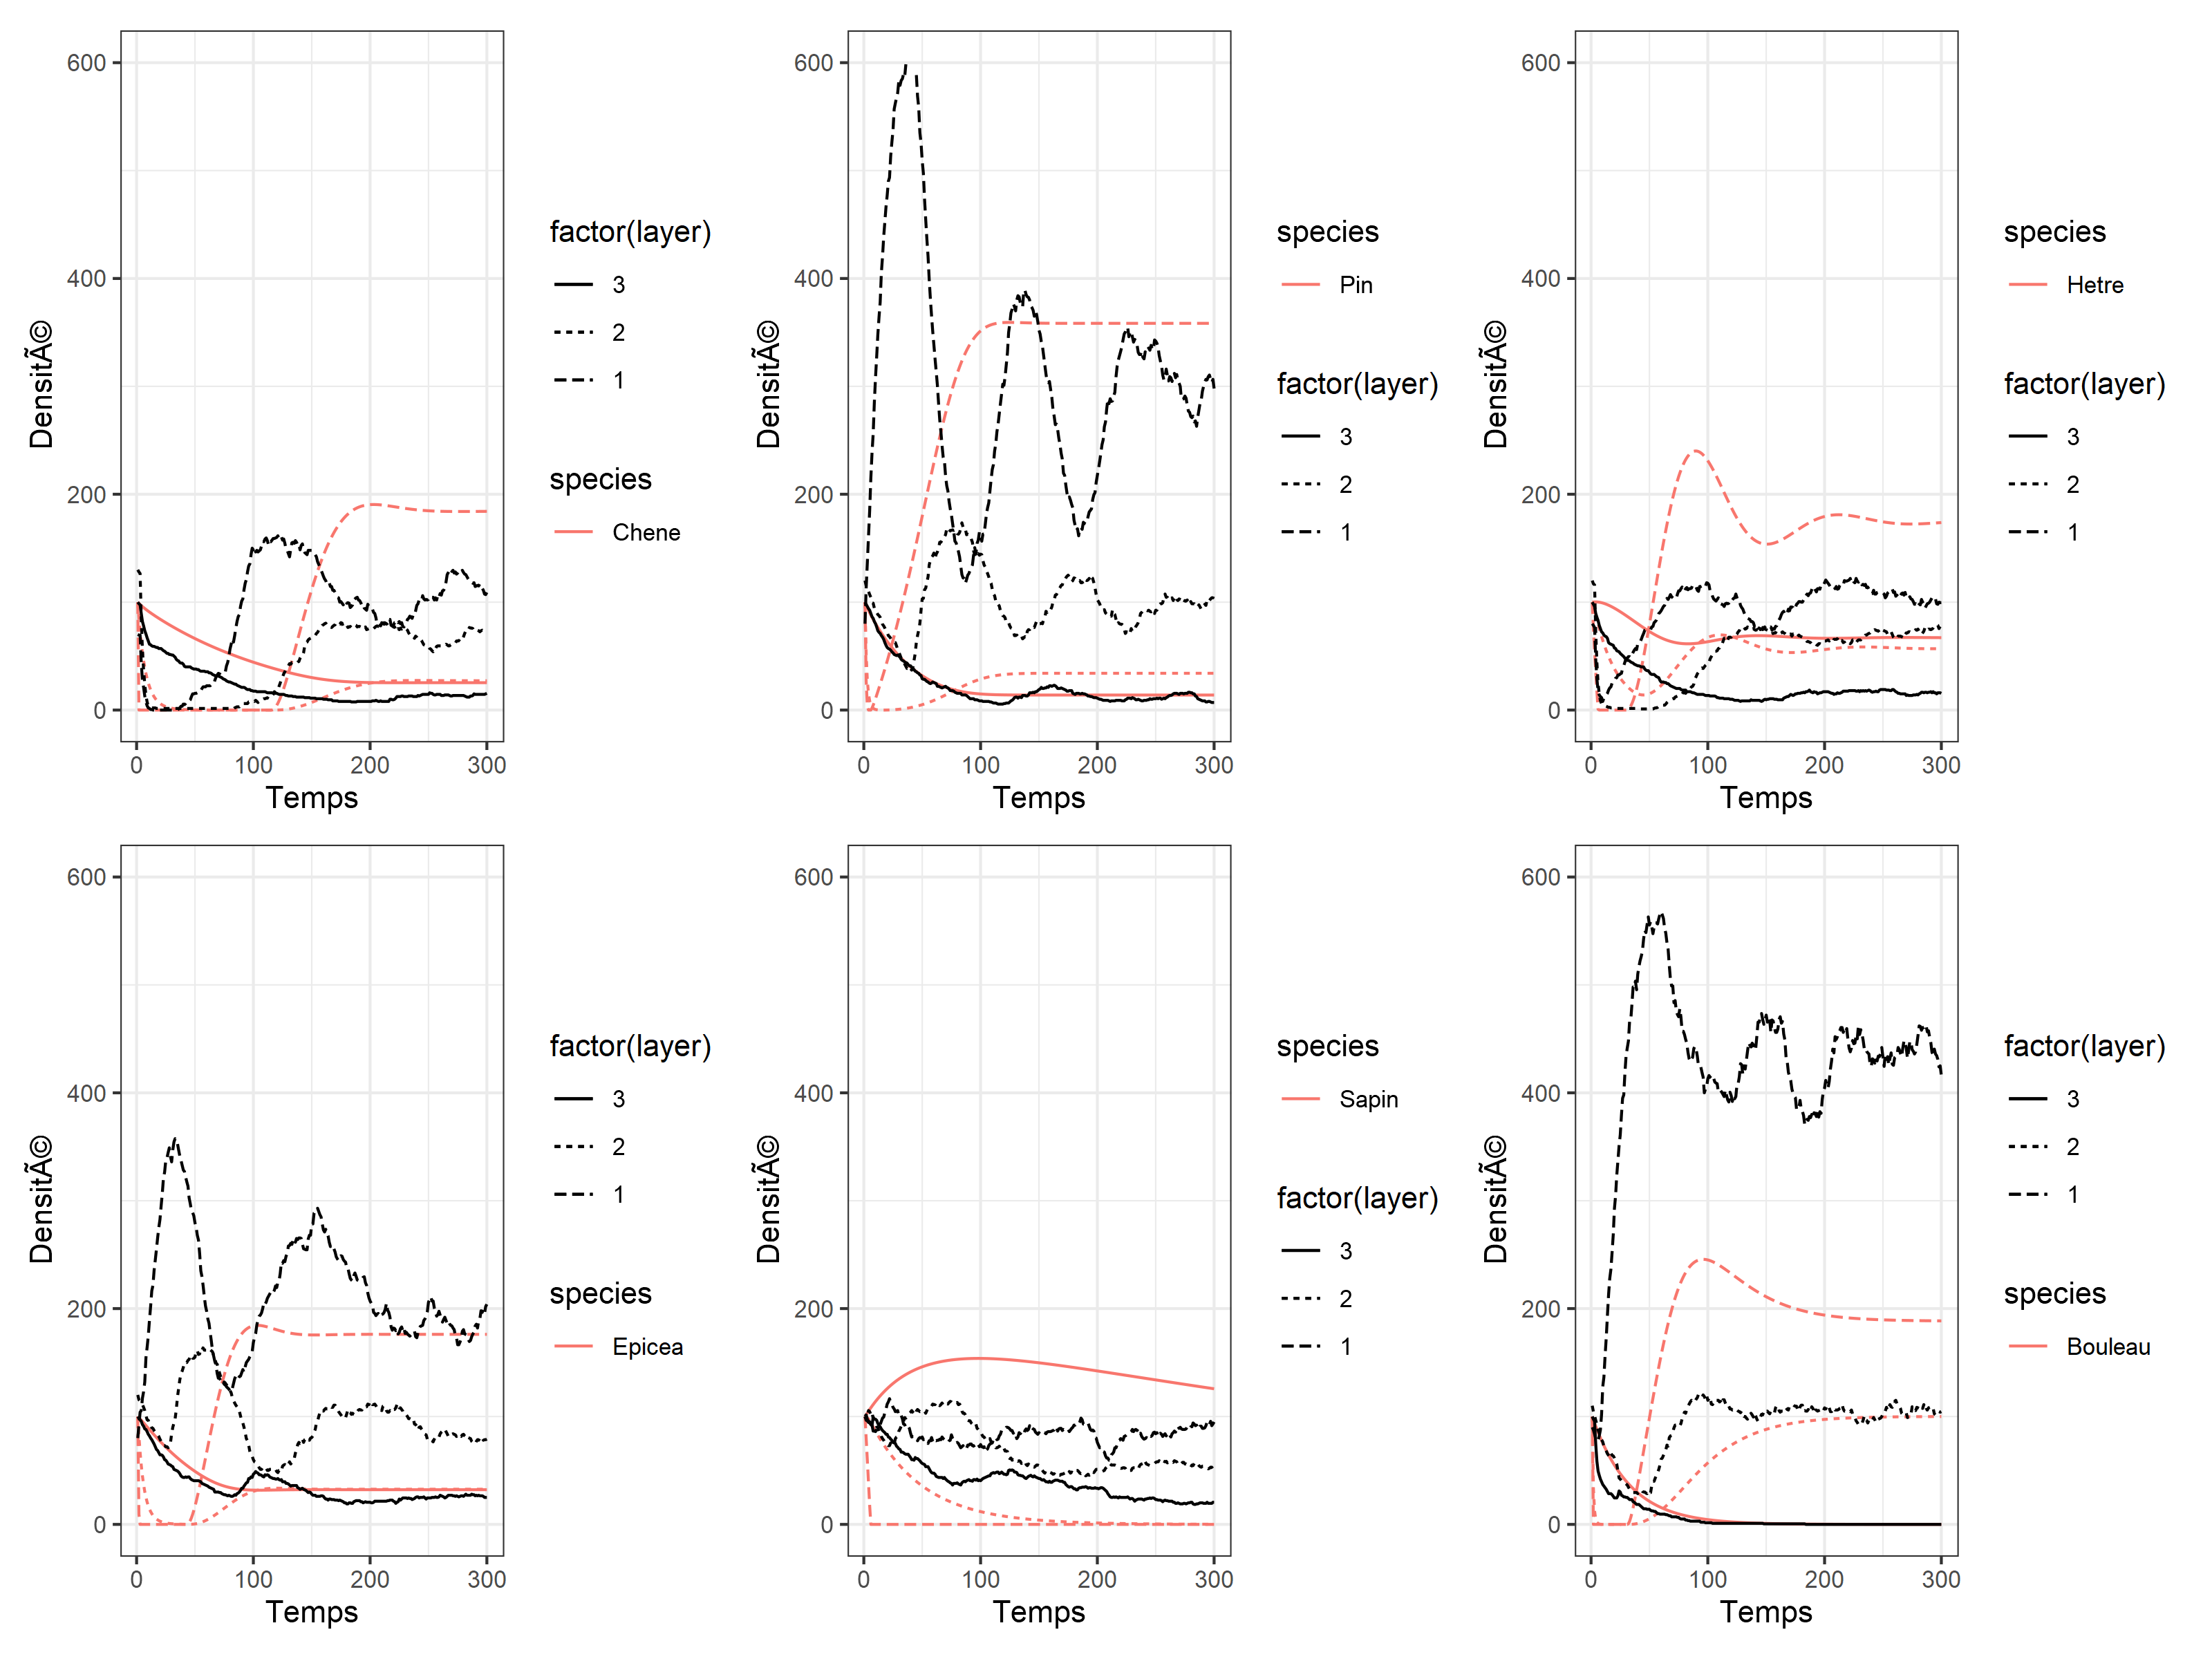
\includegraphics[width=0.8\textwidth]{Figure/plot_fit_unique.png}
    \caption{Fit Kohyama model (color) on ForCEEPS simulation (black) for individual species}
    \label{fig:my_label}
\end{figure}

\begin{figure}[H]
    \centering
    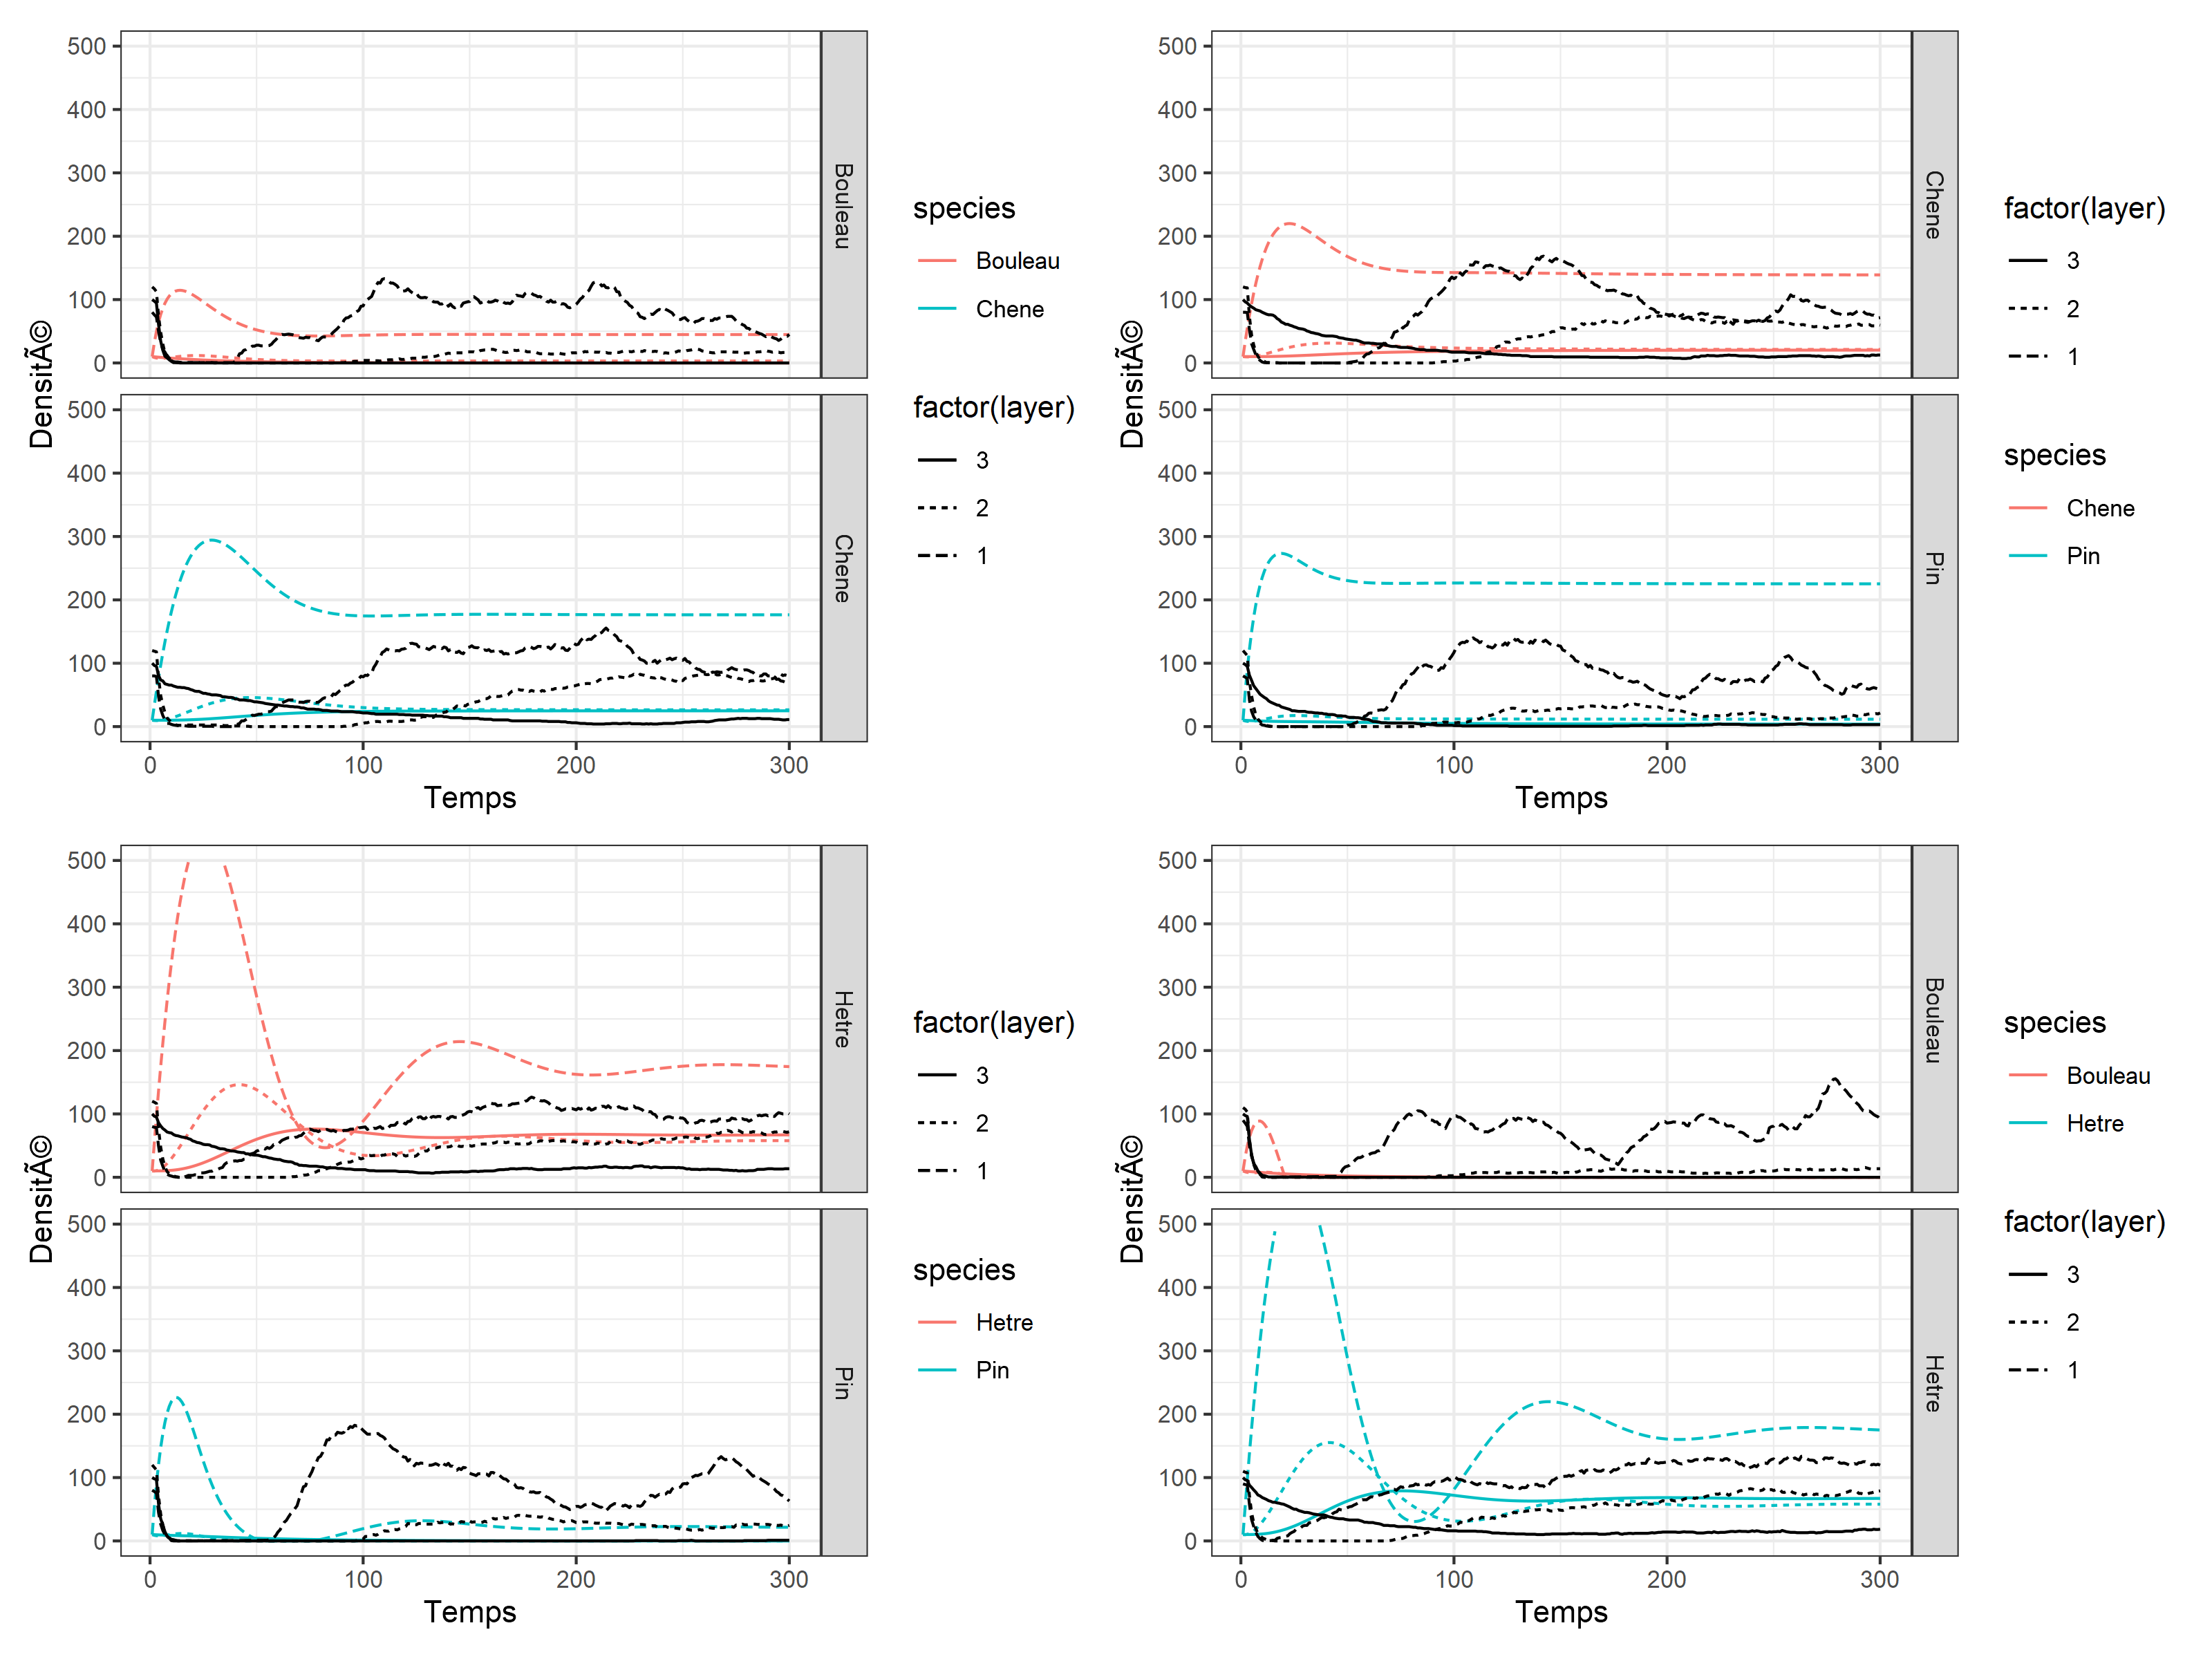
\includegraphics[width=0.8\textwidth]{Figure/plot_fit_multi.png}
    \caption{Fit Kohyama model (color) on ForCEEPS simulation (black) for mixted species stand}
    \label{fig:my_label}
\end{figure}

\begin{table}[H]
\begin{center}
    \begin{tabular}{llllllll}
    \hline
    Species & b (/ha/an) & m (/year) & g1 (/year) & g2 (/year) & LCb & LCm & LCg \\ \hline
    \textit{Abies alba}& 60 & 0.013 & 0.022 & 0.021 & 0.012 & 0.025 & 0.0013 \\
    \textit{Betula pendula} & 60 & 0.031 & 0.022 & 0 & 0.028 & 0.22 & 0.031 \\
    \textit{Fagus sylvatica} & 60 & 0.012 & 0.016 & 0.016 & 0.012 & 0.025 & 0.012 \\
    \textit{Picea abies} & 60 & 0.015 & 0.022 & 0.02 & 0.02 & 0.12& 0.015 \\
    \textit{Pinus sylvestris} & 60 & 0.023 & 0.013 & 0.012 & 0.012 & 0.22 & 0.023 \\
    \textit{Quercus pubescens} & 60 & 0.008 & 0.012 & 0.011  & 0.028 & 0.2 & 0.008 \\ \hline
    \end{tabular}
    \caption{Parameters found for the 5 species}
\end{center}
\end{table}

\section{Model dynamic}

\begin{figure}[H]
    \centering
    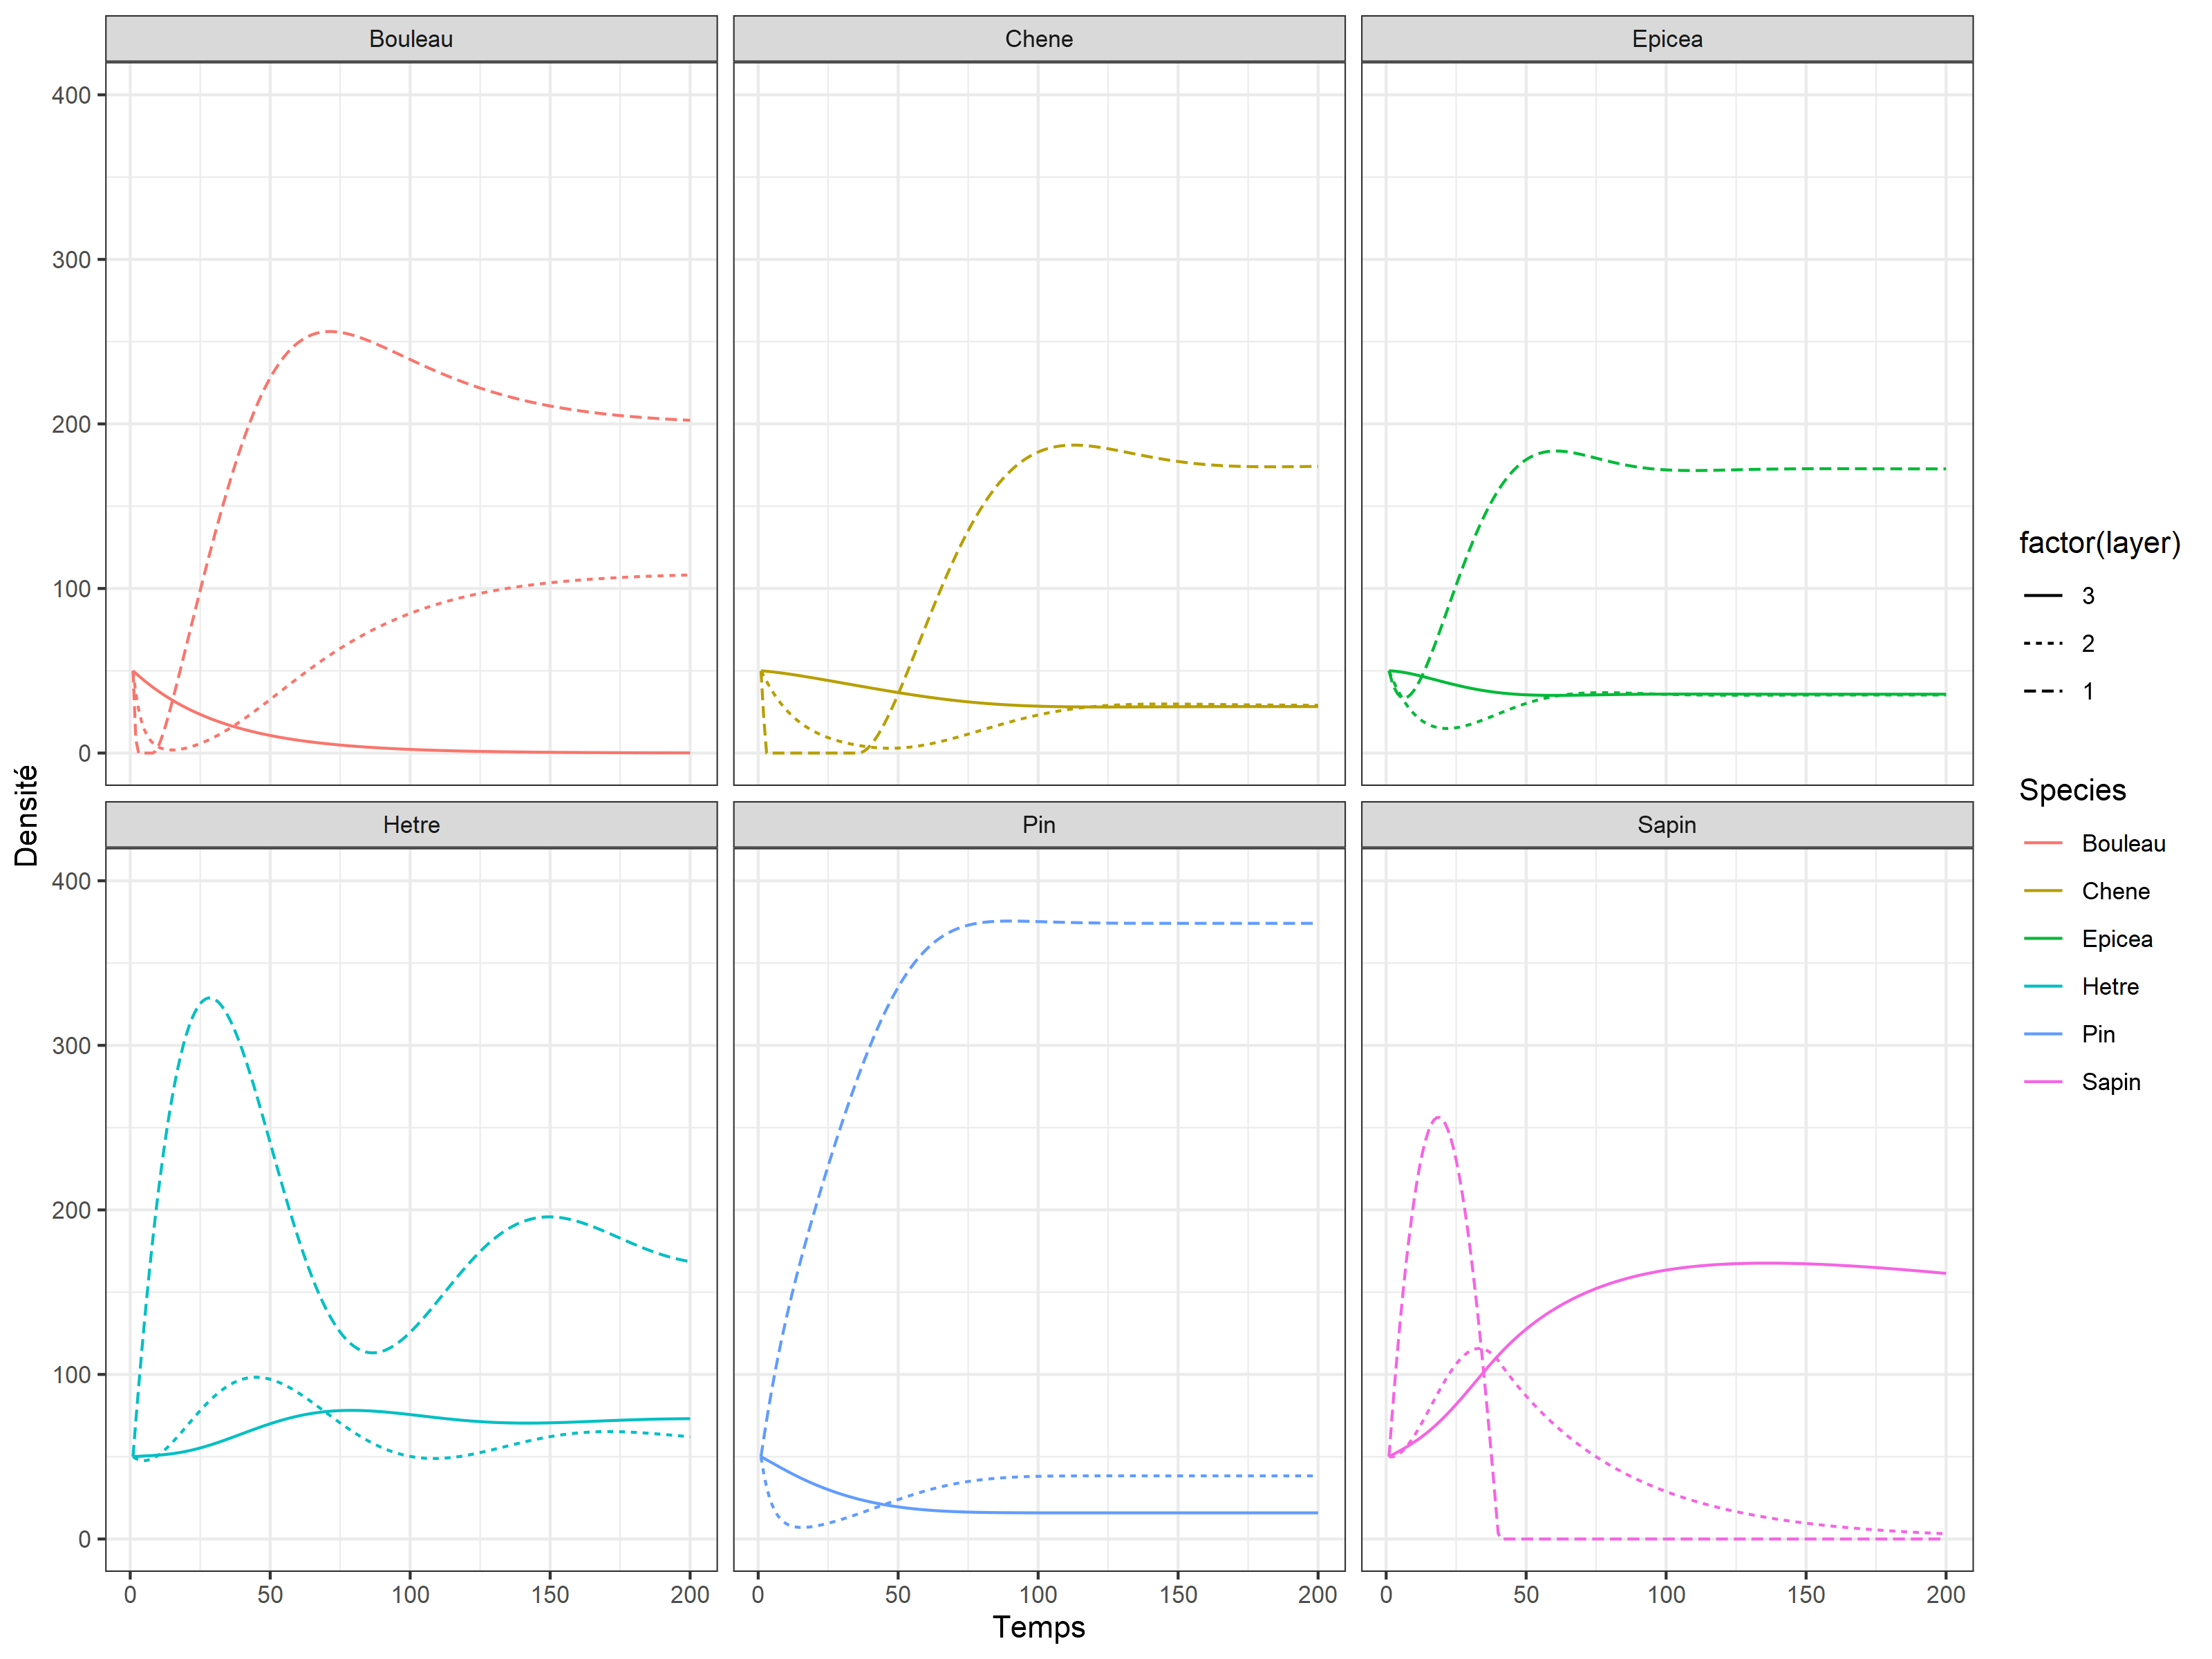
\includegraphics[width=0.8\textwidth]{Figure/Model_simple.png}
    \caption{Fit Kohyama model mono species stand}
    \label{fig:my_label}
\end{figure}

\begin{figure}[H]
    \centering
    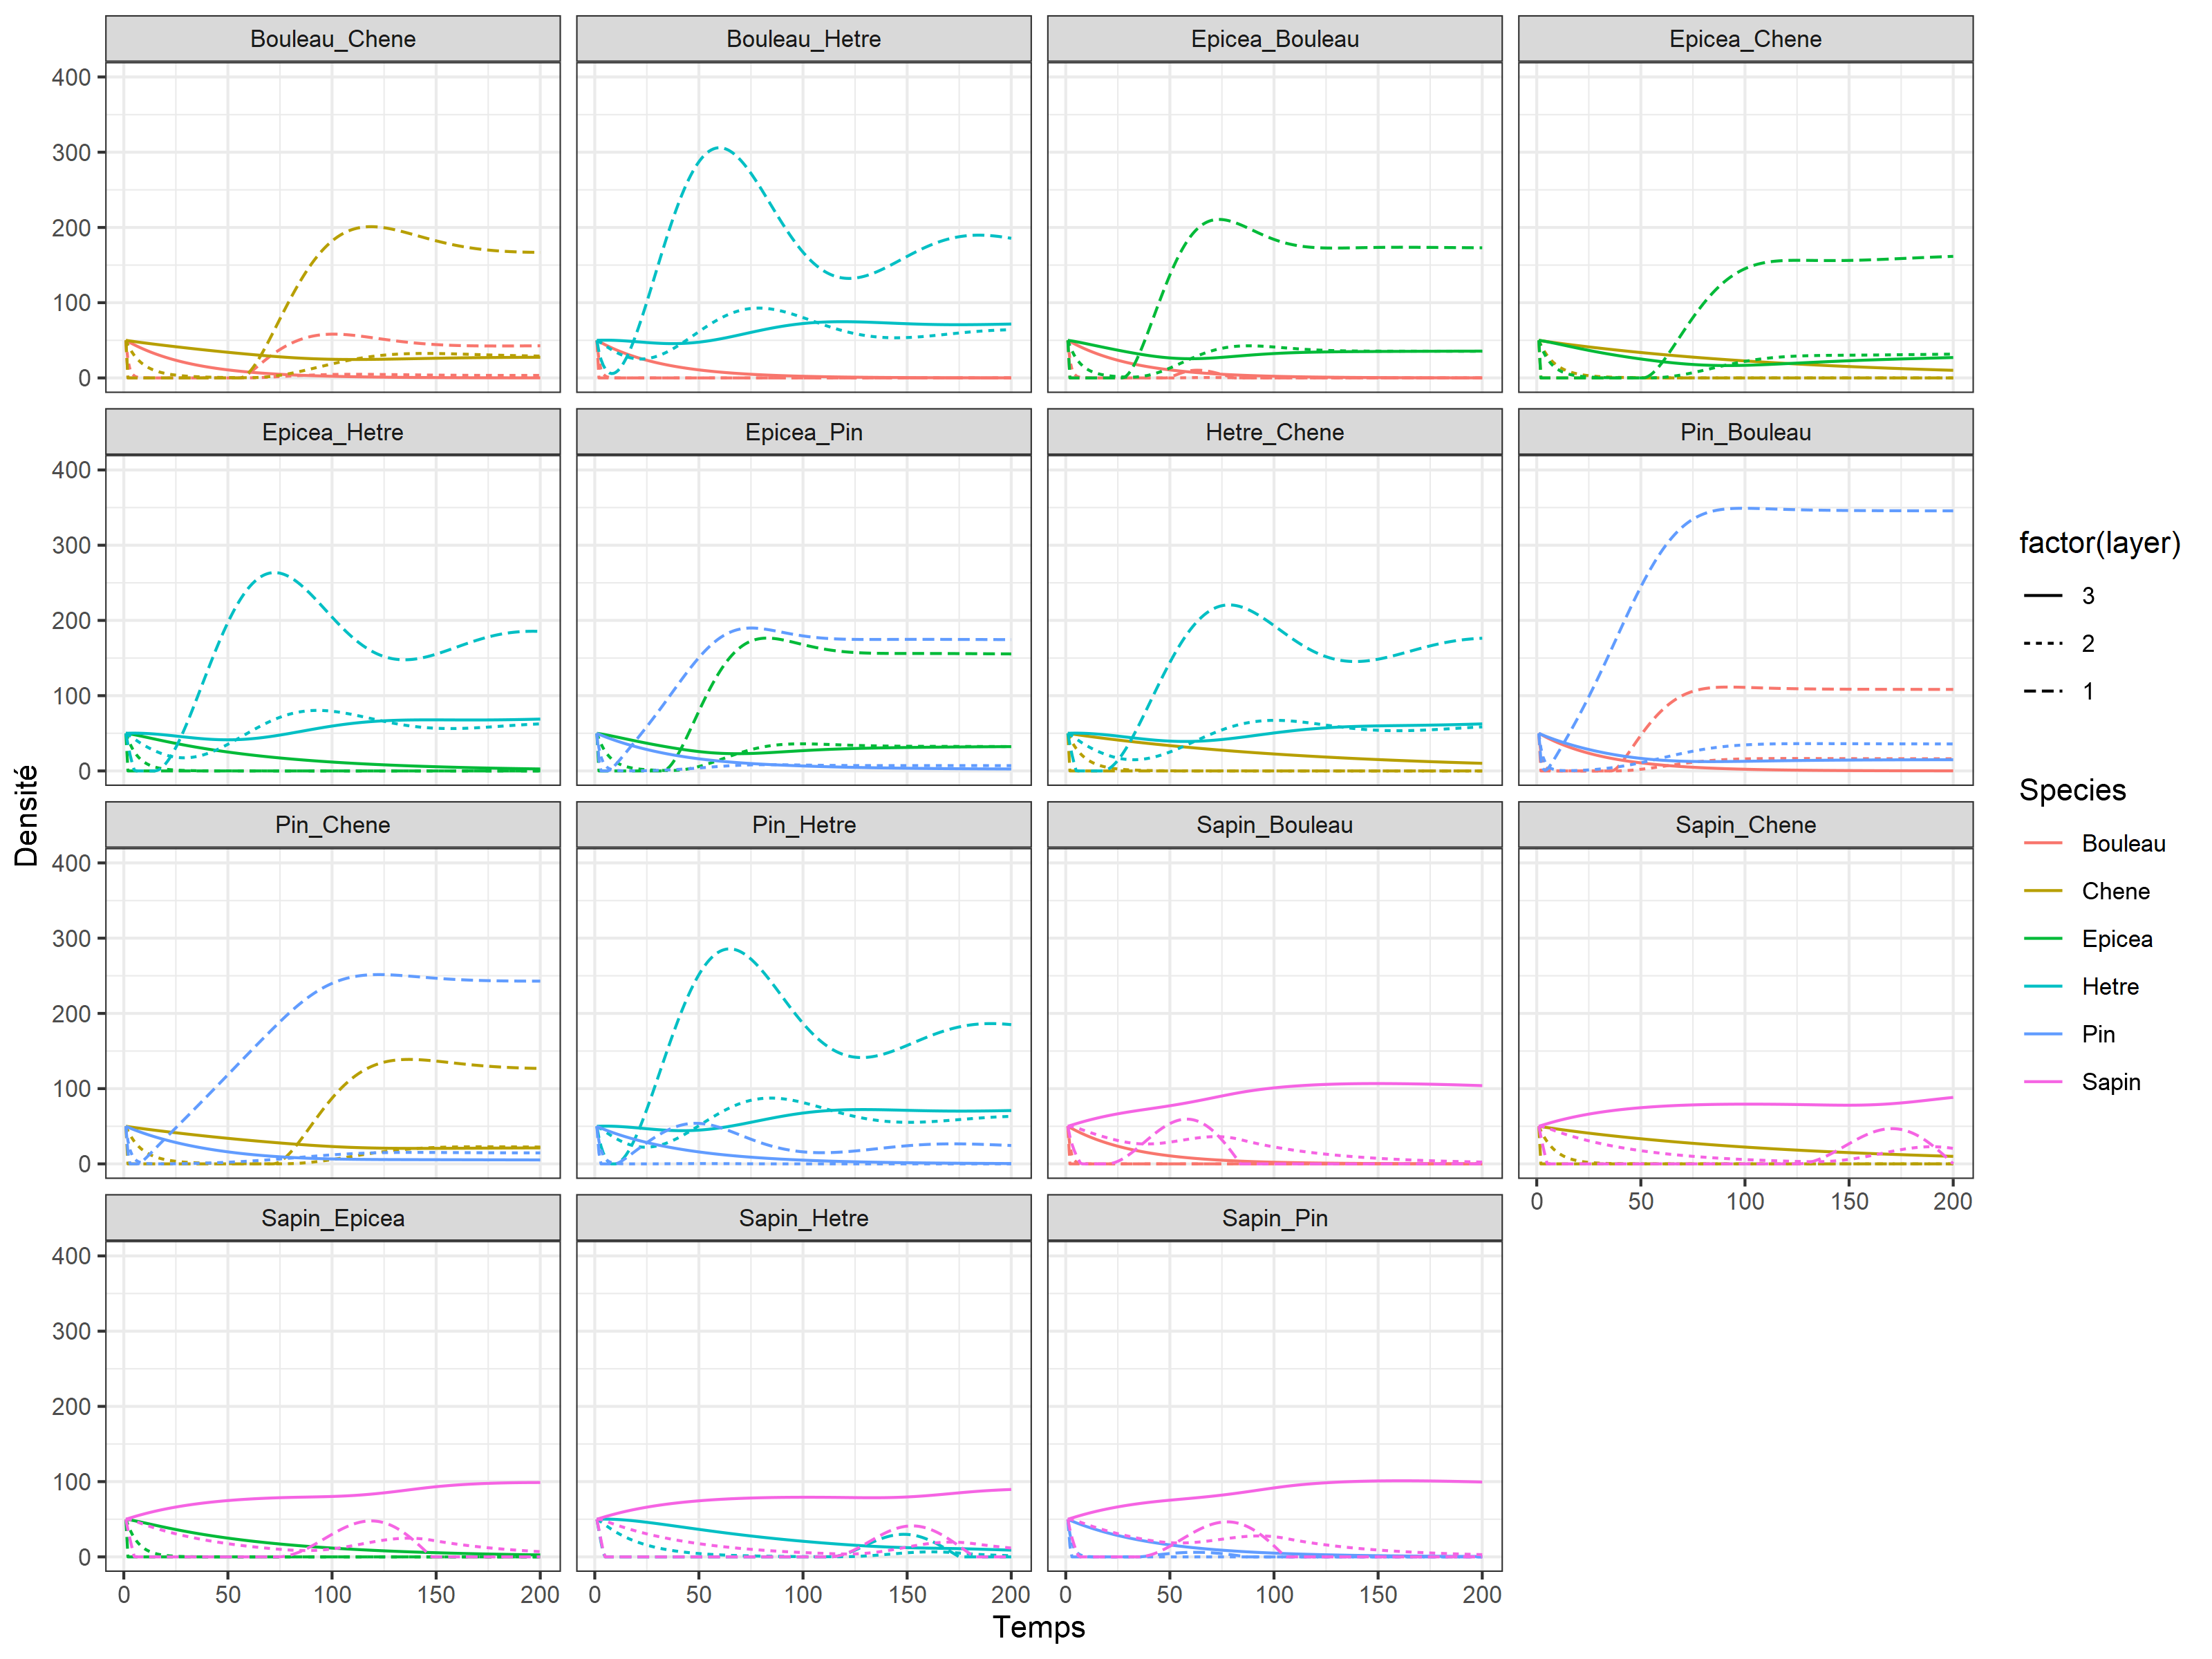
\includegraphics[width=0.8\textwidth]{Figure/Model_mixte.png}
    \caption{Fit Kohyama model for mixted species stand}
    \label{fig:my_label}
\end{figure}

\end{document}